\documentclass[main.tex]{subfiles}

\begin{document}
\section{Kirchhoffov index rezistentnosti grafu}
\label{sec:kirchhoff}

Môžeme sa pozrieť globálne na železničnú sieť podľa toho, ako jednoducho sa po nej cestuje. Požičiame si ideu z elektrických obvodov -- ak sa na každú hranu pozrieme ako na rezistor s odporom rovným jej dĺžke (čím dlhšia trasa, tým náročnejšie cestovanie), môžeme počítať tzv. rezistentnú vzdialenosť $R_{i,j}$ medzi vrcholmi $i,~j$. Čím vyššia je táto vzdialenosť, tým je prepojenie medzi týmito dvoma vrcholmi rezistentnejšie, teda v ponímaní železničných sietí horšie. Globálna hodnota pre graf, ktorá sumarizuje celkovú rezistentnosť grafu, sa nazýva Kirchhoffov index, označujeme $\mathit{Kf}(G)$, a jeho základný tvar je suma rezistentných vzdialeností pre všetky páry vrcholov. Túto hodnotu vieme vyjadriť aj nasledovne:

\begin{equation*}
	\mathit{Kf}(G) = \sum_{\substack{i, j \in V(G) \\ i < j}} R_{i,j} = n\sum_{i=1}^{n-1} \frac{1}{\lambda_i},
\end{equation*}

\noindent kde $n$ je počet vrcholov a $\lambda_i$ pre $i \in \{1, \dots, n-1\}$ sú nenulové vlastné hodnoty váhovaného Laplaciánu matice [Kinkar C. D., On the Kirchhoff Index of Graphs, 2013]. 

Pretože Kirchhoffov index interpretuje váhy hrán ako elektrické konduktivity (ako ľahko medzi nimi prechádza tok), zvolíme za váhu každej hrany inverznú hodnotu vzdialenosti (v km, pre rozumnejšiu mierku výsledku) medzi dvoma stanicami. Tým zaistíme, že čím sú stanice bližšie, tým silnejšie je medzi nimi prepojenie v grafe. 

Treba poznamenať, že Kirchhoffov index pre nesúvislé grafy je $\infty$, keďže rezistentná vzdialenosť medzi vrcholmi v dvoch rôznych komponentoch je $\infty$ (z jedného sa nedá dostať do druhého). Preto budeme v nasledujúcich analýzach pracovať iba s najväčších súvislým komponentom v slovenskej a v českej železničnej sieti.

Kirchhoffov index nie je priamo porovnávateľný medzi grafmi, keďže pracuje s počtami vrcholov a škálami váh. Keďže chceme porovnať českú a slovenskú železničnú sieť, normalizujeme rezistentnú vzdialenosť na počet všetkých dvojíc vrcholov v grafe, čím dostaneme normalizovaný Kirchhoffov index $\mathit{Kf}_n(G)$ (keďže obidve siete sú váhované vzdialenosťami, tie nemusíme normalizovať):

\begin{equation*}
	\mathit{Kf}_n(G) = \sum_{\substack{i, j \in V(G) \\ i < j}} \frac{R_{i,j}}{\binom{n}{2}} = \frac{2}{n(n-1)} \sum_{\substack{i, j \in V(G) \\ i < j}} R_{i,j} = \frac{2}{n-1}\sum_{i=1}^{n-1} \frac{1}{\lambda_i}
\end{equation*}

Môžeme teraz spočítať $\mathit{Kf}_n(G)$ pre obe siete:

\begin{align*}
		\mathit{Kf}_n(G_{\text{svk}}) &= 92.29 & \mathit{Kf}_n(G_{\text{cze}}) &= 65.99
\end{align*}

Nižší Kirchhoffov index českej siete naznačuje vyššiu celkovú konektivitu -- teda, že cestovanie medzi dvojicami staníc je v priemere efektívnejšie ako v slovenskej sieti.

Môžeme sa pokúsiť zistiť, či nevieme nájsť nižšie hodnoty tohto indexu po nejakých náhodných úpravách v železničných sieťach. Chceme však zachovať (aspoň približne) celkovú dĺžku koľajníc, aby sme simulovali, či, vzhľadom na Kirchhoffov index, by sme nevedeli nadizajnovať optimálnejšiu sieť s rovnakým rozpočtom. Pri generovaní budeme teda vychádzať z pôvodnej siete a používať upravenú verziu Pythonovskej funkcie \verb*|networkx.connected_double_edge_swap|. Algoritmus bude hľadať také štyri vrcholy $a,~b,~c,~d$, že existujú hrany $a-b$ a $c-d$, neexistujú hrany $a-d$ a $b-c$ a všetky vzdialenosti $a-b,~b-c,~c-d,d-a$ sú približne rovnaké, čiže efektívne tvoria (koso)štvorec. Následne vymažeme hrany $a-b$ a $c-d$ a pridáme hrany $a-d$ a $b-c$ (keďže $a,~b,~c,~d$ tvoria skoro štvorec, súčet dĺžok všetkých koľajníc by sa nemusel veľmi zmeniť). Ak sa však graf touto zmenou rozpadne na dva komponenty, vrátime ju naspäť.  Vizualizáciu dvoch takýchto výmen môžeme vidieť na obr. \ref{fig:double_edge_swap}.

\begin{figure}
	\centering
	
	\begin{subfigure}{0.45\linewidth}
		\centering
		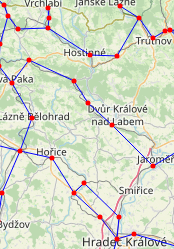
\includegraphics[width=0.6\linewidth]{images/before_swap.png}
	\end{subfigure}
	\begin{subfigure}{0.45\linewidth}
		\centering
		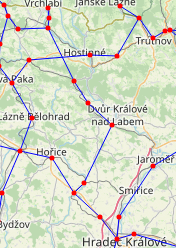
\includegraphics[width=0.6\linewidth]{images/after_swap.png}
	\end{subfigure}
	
	\caption{Vizualizácia dvoch výmen v našom modifikovanom \texttt{networkx.connected\_double\_edge\_swap} algoritme. Tieto dve výmeny spolu s dvomi ďalšími mali za následok nižšiu hodnotu Kirchhoffovho indexu pre českú sieť.}
	\label{fig:double_edge_swap}
\end{figure}

Tento algoritmus zopakujeme 100-krát pre Slovensko a pre Česko. V každom sa pokúsime urobiť približne 100 výmen, no keďže kladieme tvrdé podmienky na výber hrán na výmenu, v priemere každý beh algoritmu spravil okolo 9 výmen (čiže siete sme modifikovali iba zľahka). Môžeme sa pozrieť na rozdelenie Kirchhoffovho indexu (vo forme jadrového odhadu hustoty) v týchto modifikovaných grafoch spolu so skutočnými hodnotami (obr. \ref{fig:kirchhoff_random_networks}).

\begin{figure}
	\centering
	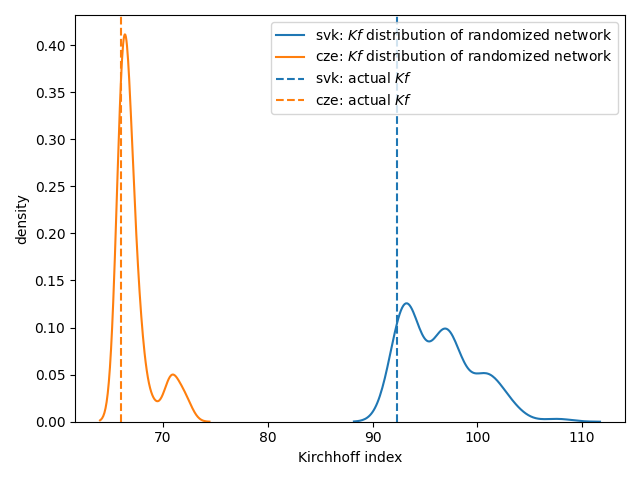
\includegraphics[width=0.7\textwidth]{images/kde_kirchhoff_randomized.png}
	\caption{Jadrový odhad hustoty Kirchhoffovho indexu na modifikovaných železničných sieťach spolu so skutočnými hodnotami.}
	\label{fig:kirchhoff_random_networks}
\end{figure}

Vidíme, že skutočné hodnoty indexu sa nachádzajú v ľavých častiach týchto distribúcií. Kirchhoffov index pre slovenskú železničnú sieť bol nižší od indexov 99\% modifikovaných sietí, pre českú sieť bol nižší od 97\%. Môžeme teda usúdiť, že pre aktuálne rozloženie staníc a súčet dĺžok koľajníc sú obidve siete vzhľadom na normalizovaný Kirchhoffov index pomerne optimalizované, čo naznačuje, že boli dobre nadizajnované. 

\subsection{Centralita efektívnej rezistencie}

Dôležitým meradlom kvality verejnej dopravy je jej odolnosť voči výpadkom spojení. Zadefinujme si tzv. centralitu efektívnej rezistencie vzhľadom na vrcholy (označíme $R(v_i, G)$) a vzhľadom na hranu $R(e_{i,j}, G)$ [Cornaro A. a Grechi D., Evaluation of Railway Systems: A Network Approach, 2023]:

\begin{align*}
	R(v_i, G) &=  \frac{\mathit{Kf}_n(G'_{v_i}) - \mathit{Kf}_n(G)}{\mathit{Kf}_n(G)}, \\
	R(e_{i,j}, G) &=  \frac{\mathit{Kf}_n(G'_{e_{i,j}}) - \mathit{Kf}_n(G)}{\mathit{Kf}_n(G)},
\end{align*}

\noindent kde $G'_{v_i}$ je vytvorený z grafu $G$ odstránením vrchola $v_i$ a všetkých hrán s ním incidentných a $G'_{e_{i,j}}$ je vytvorený z grafu $G$ odstránením hrany $e_{i,j}$. Jedná sa teda o relatívnu zmenu v normalizovanom Kirchhofovom indexe po odstránení nejakej súčasti grafu.

V našom kontexte môžeme interpretovať túto centralitu ako citlivosť rezistentnosti grafu na výpadok spojenia/stanice (napr. z dôvodu rekonštrukcie, vykoľajenia vlaku alebo z iných nepredvídateľných dôvodov). Môžeme napríklad očakávať, že keď odstránime dôležitú prestupnú stanicu, doprava po železničnej sieti bude náročnejšia, keďže budeme musieť robiť obchádzky. 

Vizualizujme túto centralitu pre Česko a Slovensko. Farebná škála (individuálna pre každú vizualizáciu) ide od čiernej (najnižšia centralita) cez fialovú po žltú (najvyššia centralita). Mosty a artikulácie sú vyznačené modrou, keďže tie majú nekonečnú centralitu rezistencie -- obr. \ref{fig:resistance_svk} a obr. \ref{fig:resistance_cze}. 

\begin{figure}
	\centering
	
	\begin{subfigure}{\linewidth}
		\centering
		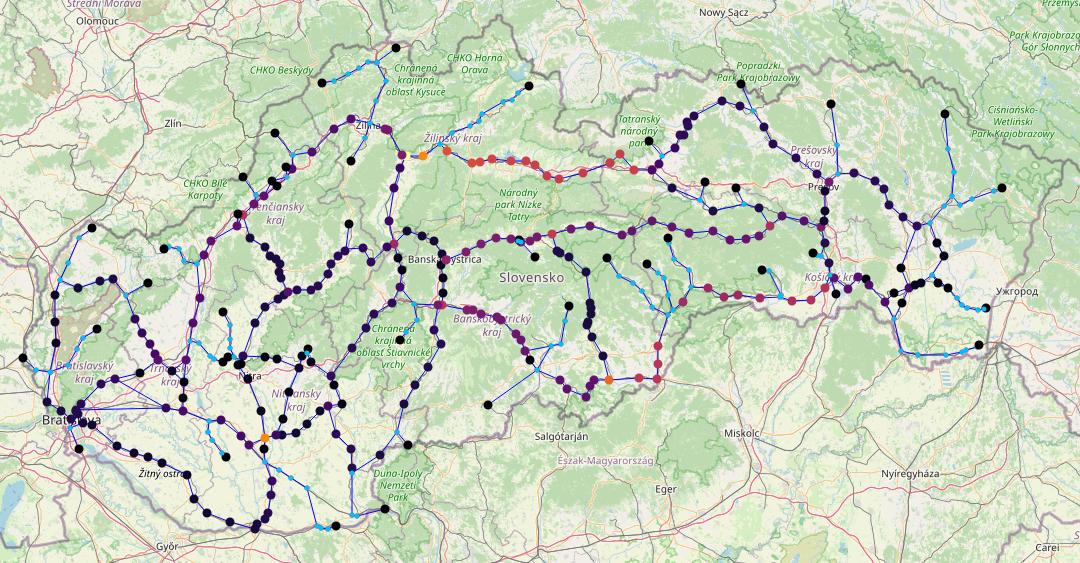
\includegraphics[width=\textwidth]{images/svk_vertex_resistance.png}
	\end{subfigure}
	
	\vspace{0.5cm}
	
	\begin{subfigure}{\linewidth}
		\centering
		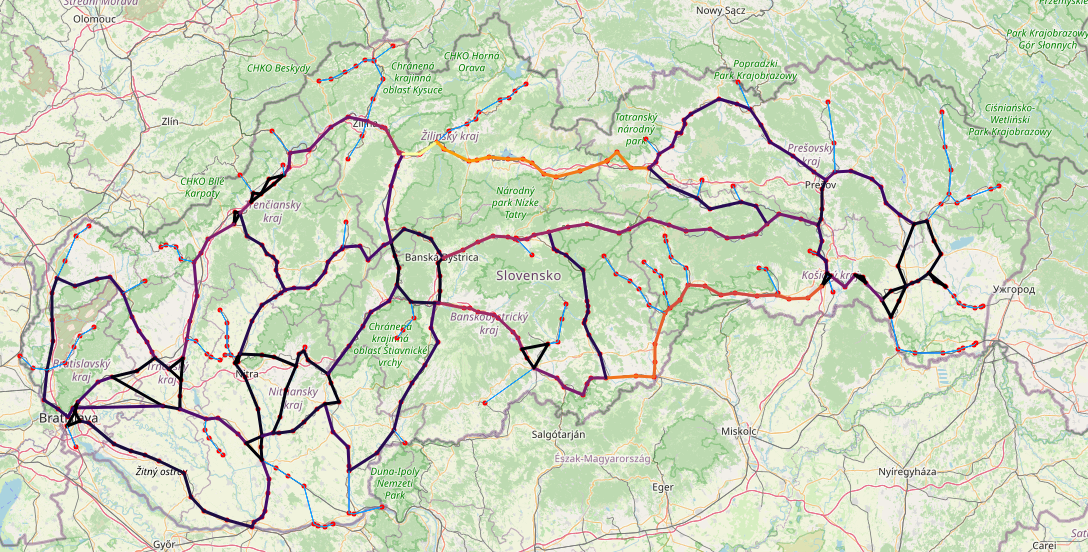
\includegraphics[width=\textwidth]{images/svk_edge_resistance.png}
	\end{subfigure}
	
	\caption{Centralita efektívnej rezistencie vzhľadom na vrcholy (hore) a vzhľadom na hrany (dole) pre slovenskú železničnú sieť.}
	\label{fig:resistance_svk}
\end{figure}

\begin{figure}
	\centering
	
	\begin{subfigure}{\linewidth}
		\centering
		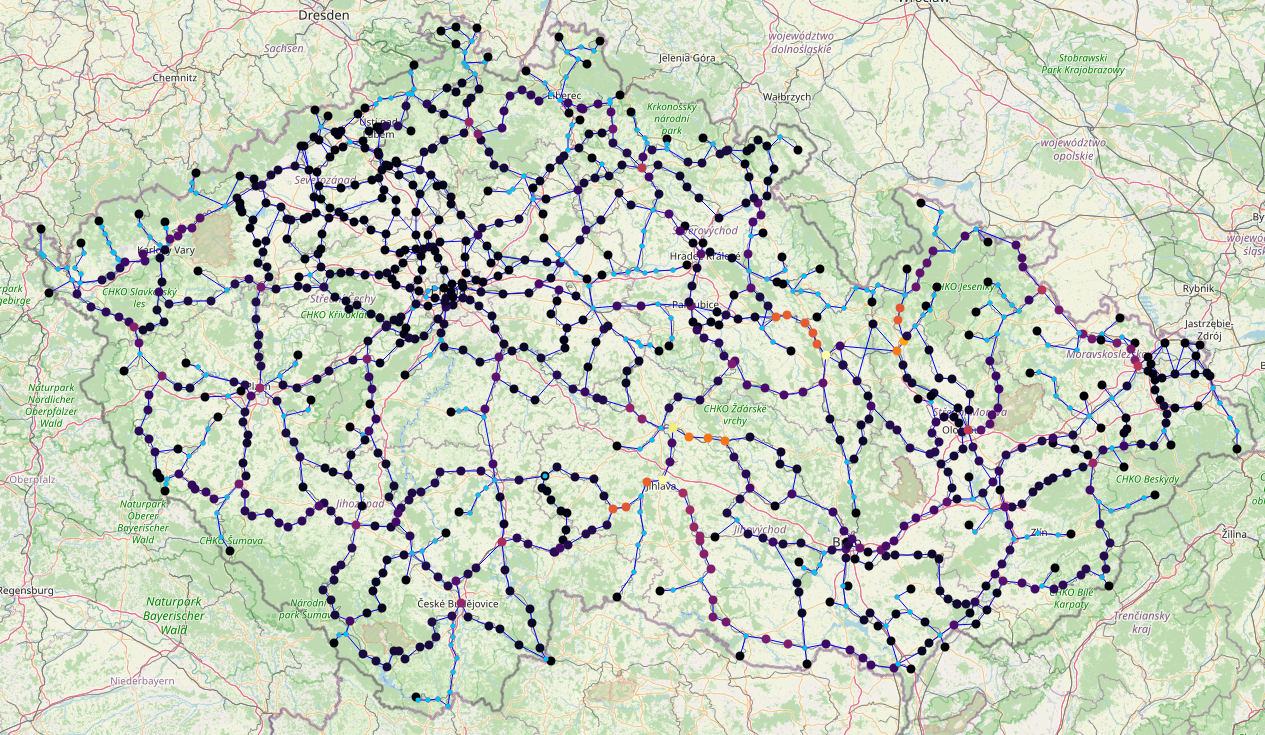
\includegraphics[width=\textwidth]{images/cze_vertex_resistance.png}
	\end{subfigure}
	
	\vspace{0.5cm}
	
	\begin{subfigure}{\linewidth}
		\centering
		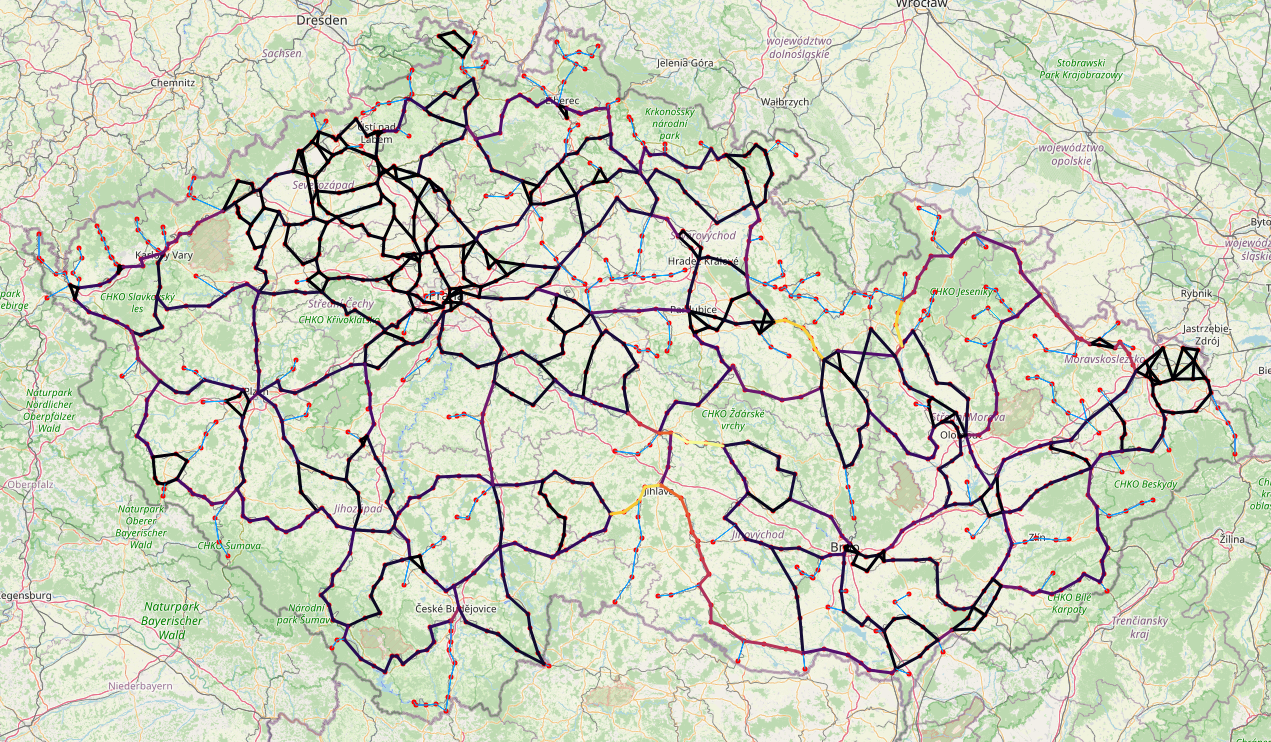
\includegraphics[width=\textwidth]{images/cze_edge_resistance.png}
	\end{subfigure}
	
	\caption{Centralita efektívnej rezistencie vzhľadom na vrcholy (hore) a vzhľadom na hrany (dole) pre českú železničnú sieť.}
	\label{fig:resistance_cze}
\end{figure}

Môžeme odpozorovať, že naša interpretácia sedí s pozorovanými výsledkami. Vrcholy s vysokovou centralitou efektívnej rezistencie sú často stanice, ktoré spájajú viacero traktov, ako napríklad Vrútky a Šurany na Slovensku, Plzeň a Jihlava v Česku. Keď sa pozrieme na hranovú centralitu, môžeme vidieť, že pre Slovensko sú kritické tri trakty prepájajúce východ so stredom/západom (Vrútky -- Poprad, Košice -- Zvolen, Kysak -- Banská Bystrica). Jedná sa teda o pomerne dôležité trakty, ktorých porušenie by malo veľký dopad na celú sieť a teda jedná sa o časť siete, ktorá nie je veľmi odolná voči výpadkom. Podobnú seperáciu vidíme aj v Česku, medzi juhovýchodom a stredom/západom. Nájdeme tu však iba jeden dlhý kritický trakt (Břeclav -- okolie Jihlavy) a dva pomerne krátke (Choceň -- Třebovice, Postřemelov -- Hanušovice). Česká sieť je teda náchylná na výpadky v tejto oblasti.

Pozrime sa však na porovnanie distribúcií týchto centralít (obr. \ref{fig:resistance_distr}). Môžeme si všimnúť, že distribúcia v oboch prípadoch má pre Slovensko omnoho ťažší chvost. Z týchto hodnôt môžeme usúdiť, že napriek tomu, že sme identifikovali kritické trakty v Česku aj na Slovensku, Slovensko je ďaleko náchylnejšie na výpadok nejakej stanice alebo spojenia. Výpadok stanice v slovenskej sieti má za následok zvýšenie rezisentnosti (\enquote{komplikovanosti} dopravy) v priemere o 7\%, zatiaľ čo v Česku to je v priemere o 1\%. Podobné správanie vidíme aj pri výpadkoch spojení medzi stanicami. Táto štatistika ukazuje, že česká sieť je lepšie pripravená na jej porušenie ako slovenská.

\begin{figure}
	\centering
	
	\begin{subfigure}{\linewidth}
		\centering
		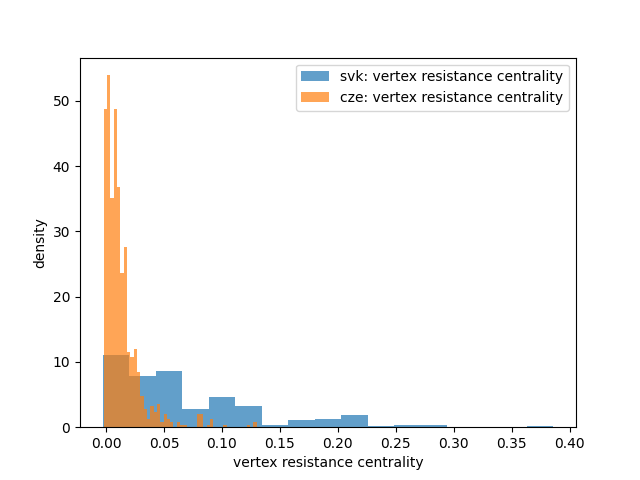
\includegraphics[width=0.9\textwidth]{images/vertex_resistance_distribution.png}
	\end{subfigure}
	
	\vspace{0.5cm}
	
	\begin{subfigure}{\linewidth}
		\centering
		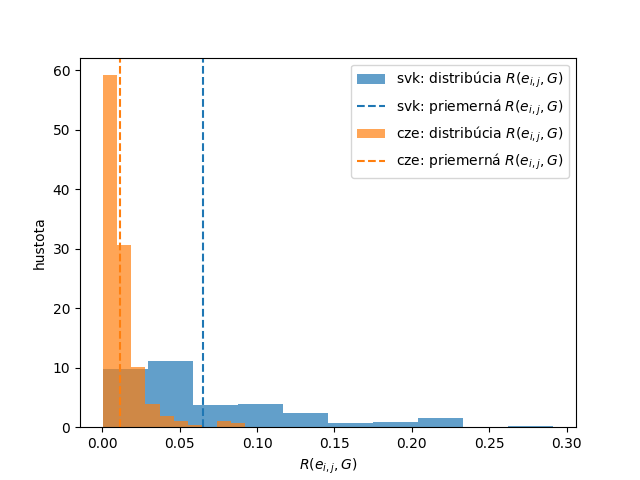
\includegraphics[width=0.9\textwidth]{images/edge_resistance_distribution.png}
	\end{subfigure}
	
	\caption{Distribúcie centralít efektívnej rezistencie vzhľadom na vrchol (hore) a vzhľadom na hranu (dole), spolu s ich priemermi.}
	\label{fig:resistance_distr}
\end{figure}






	
\end{document}